\documentclass[12pt]{article}

%% Language and font encodings
\usepackage[french]{babel}
\usepackage[utf8]{inputenc}
\usepackage[T1]{fontenc}

\usepackage{csquotes}
%\usepackage{fontspec}
\usepackage{xltxtra}
%\setmathfont{texgyretermes-math.otf}
\setmainfont[Ligatures=Rare]{Linux Libertine O}%

\usepackage{float}

\setlength{\parindent}{1em}
%\setlength{\parskip}{1ex plus 0.5ex minus 0.2ex}
\newcommand{\hsp}{\hspace{20pt}}
\newcommand{\HRule}{\rule{\linewidth}{0.5mm}}

\usepackage{algorithm}
\usepackage[noend]{algpseudocode}
\algnewcommand{\algorithmicand}{\textbf{ and }}
\algnewcommand{\algorithmicor}{\textbf{ or }}
\algnewcommand{\OR}{\algorithmicor}
\algnewcommand{\AND}{\algorithmicand}
\algnewcommand\algorithmicforeach{\textbf{for each}}
\algdef{S}[FOR]{ForEach}[1]{\algorithmicforeach\ #1\ \algorithmicdo}
\newcommand{\myfrac}[2]{\frac{\displaystyle {#1}}{\displaystyle {#2}}}

%% Sets page size and margins
\usepackage[a4paper,top=3cm,bottom=2cm,left=3cm,right=3cm,marginparwidth=1.75cm]{geometry}

%% Useful packages
\usepackage{amsmath}
\usepackage{amssymb}
\usepackage{graphicx}
\usepackage{subcaption}
\usepackage[colorinlistoftodos]{todonotes}
\usepackage[colorlinks=true, allcolors=blue]{hyperref}
\usepackage{graphicx}

\usepackage{enumitem}

\usepackage{listings}
\lstset{language=Python} 

\usepackage{colortbl}

\usepackage[htt]{hyphenat}

\interfootnotelinepenalty=10000
\usepackage[bottom]{footmisc}

\usepackage{fancyvrb,cprotect}

%\usepackage[most]{tcolorbox}
%\definecolor{block-gray}{gray}{0.85}
%\newtcolorbox{blockquote}{colback=block-gray,grow to right by=-1mm,grow to left by=-1mm,boxrule=0pt,boxsep=0pt,breakable}

%% equations
\usepackage{amsthm}
\usepackage[retainorgcmds]{IEEEtrantools}

%% theorem and proposition
\newtheorem{prop}{Proposition}
\newtheorem*{prop*}{Proposition}
\newtheorem{thm}{Théorème}

\newenvironment{myproof}[1][\proofname]{\proof[#1]\mbox{}\\*}{\endproof}

%% references shortcuts
\usepackage{suffix}
\renewcommand{\eqref}[1]{équation~\ref{#1}}
\newcommand{\algoref}[1]{algorithme~\ref{#1}}
\newcommand{\figref}[1]{figure~\ref{#1}}
\newcommand{\tabref}[1]{tableau~\ref{#1}}
\newcommand{\secref}[1]{section~\ref{#1}}
\newcommand{\probref}[1]{problème~\ref{#1}}
\newcommand{\propref}[1]{proposition~\ref{#1}}
\newcommand{\theoremref}[1]{théorème~\ref{#1}}
\newcommand{\chapref}[1]{chapitre~\ref{#1}}
\newcommand{\appref}[1]{annexe~\ref{#1}}
\WithSuffix\newcommand\algoref*[1]{algorithme~\ref{#1} p.~\pageref{#1}}
\WithSuffix\newcommand\figref*[1]{figure~\ref{#1} p.~\pageref{#1}}
\WithSuffix\newcommand\eqref*[1]{équation~\ref{#1} p.~\pageref{#1}}
\WithSuffix\newcommand\tabref*[1]{tableau~\ref{#1} p.~\pageref{#1}}
\WithSuffix\newcommand\secref*[1]{section~\ref{#1} p.~\pageref{#1}}
\WithSuffix\newcommand\probref*[1]{problème~\ref{#1} p.~\pageref{#1}}
\WithSuffix\newcommand\propref*[1]{proposition~\ref{#1} p.~\pageref{#1}}
\WithSuffix\newcommand\chapref*[1]{chapitre~\ref{#1} p.~\pageref{#1}}

\usepackage[backend=biber,style=authoryear-comp,uniquename=init,firstinits=true,
            %% "et al" pour > deux auteurs, & pour exactement 2
            uniquelist=false,maxcitenames=2,mincitenames=1,maxbibnames=99,
            isbn=false,url=false,doi=false
]{biblatex}

\DefineBibliographyExtras{french}{\renewcommand*\mkbibnamefamily[1]{#1}}
\renewcommand{\cite}{\parencite}
\renewcommand*{\nameyeardelim}{\addcomma \addnbspace}
% \renewcommand*{\multinamedelim}{\space} % fait le contraire de ce qu'on veut
\renewcommand*{\revsdnamedelim}{}
\renewcommand*\finalnamedelim{ \& }

\DefineBibliographyExtras{french}{\restorecommand\mkbibnamelast}

\DeclareNameAlias{default}{last-first}
\DeclareNameAlias{sortname}{last-first}

% Supprimer les guillemets dans les titres
\DeclareFieldFormat[article,incollection,unpublished,inproceedings]{title}{#1}

% Espaces insécables dans les citations et la bibliographie (noms de
% conférences) ?

\usepackage{xpatch}
\usepackage{xstring}
%\xpatchbibmacro{series+number}{\addspace}{\addnbspace}{}{}

\renewbibmacro*{series+number}{%
  \setunit*{\addnbspace}%
  \printfield{series}%
  \printfield{number}%
  \newunit}

\AtBeginDocument{ %Bizarrerie unicode-math
  \DeclareMathOperator{\mmin}{\mathrm{min}}
  \DeclareMathOperator{\mmax}{\mathrm{max}}
  \DeclareMathOperator{\eexp}{\mathrm{exp}}
  \DeclareMathOperator{\argmin}{\text{argmin}}
  \newcommand{\gargmin}[2]{\argmin_{#1}\left\{{#2}\right\} }
  \DeclareMathOperator{\prox}{\mathrm{prox}}
  \newcommand{\proxg}[3]{\prox_{\frac{#1}{#2}{#3}}}
}

\makeatletter
\newcommand*{\transpose}{%
  {\mathpalette\@transpose{}}%
}
\newcommand*{\@transpose}[2]{%
  % #1: math style
  % #2: unused
  \raisebox{0.2em}{$\m@th#1\intercal$}%
}
\makeatother

\newcommand{\tr}[1]{ {#1}^{\! \transpose}}

\xpatchbibmacro{textcite}{\addcoma}{}{}{}

\addbibresource{references.bib}

\usepackage{array,multirow}
\addto\captionsfrench{\def\tablename{TABLEAU}}


\begin{document}

\begin{titlepage}
  \begin{center}

      \makebox[0.5\textwidth][c]{%
        
\includegraphics[width=0.33\textwidth]{images/sorbonne.png}%
    }%

    \vspace{4cm}
    % Title
    \HRule \\[0.4cm]
    { \huge \bfseries REDS - Projet Boson de Higgs\\[0.4cm] }

      \textsc{\LARGE Rapport}\\[0.4cm]

    \HRule \\[0.4cm]

    % Author and supervisor
    \begin{minipage}{0.4\textwidth}
      \begin{flushleft} \large
        Kim-Anh Laura \textsc{Nguyen}\\
        Keyvan \textsc{Beroukhim} \\
        Master 2 DAC \\
        Promo 2019-2020 \\
      \end{flushleft}
    \end{minipage}
    \begin{minipage}{0.5\textwidth}
      \begin{flushright} \large
          \emph{Enseignant :} Olivier \textsc{Schwander} \\
      \end{flushright}
    \end{minipage}

      \vspace{2cm}


  \end{center}
  %\end{sffamily}
\end{titlepage}
%\maketitle

\newpage

\section{Introduction}

Nous souhaitons détecter la présence du boson de Higgs dans des données simulées
dans le but de reproduire le comportement de l'expérience ATLAS. Il s'agit d'un
problème de détection d'évènement, ou classification binaire, dans lequel les
deux classes sont :

\begin{itemize}
    \item \emph{background}
    \item \emph{tau tau decay of a Higgs boson}
\end{itemize}

Les données sont issues du projet Kaggle \emph{ATLAS Higgs Boson Machine Learning Challenge
2014}. 

\section{Analyse préliminaire des données}

La base de données est constituée de 818238 évènements simulés. Chaque évènement
est défini par 30 attributs numériques et un label à prédire. \\

Les données sont composées à \textbf{34\% de labels positifs} (les
\emph{signaux}) et à 66\% de labels négatifs (le \emph{background}). Les classes
ne sont pas suffisamment déséquilibrées pour gêner l'entraînement. Par ailleurs,
la métrique propre à cette tâche, nommée \emph{AMS}, nous est imposée. Le choix
habituel de la mesure d'évaluation à utiliser pour prendre en compte ce
déséquilibre ne se pose donc pas. \\

\subsection{Distribution des variables}

La \figref{img:hist-sample} contient les histogrammes de répartition des valeurs
de quelques variables, en omettant les valeurs manquantes. Nous constatons que
\textbf{toutes les variables ne suivent pas le même type de distribution}. Or, les
algorithmes d'apprentissage se comportent généralement mieux avec une
distribution des données équilibrée. Dans ce dataset, de nombreuses variables
ont une distribution exponentielle décroissante (e.g \texttt{DER\_MASS\_VIS} sur
la \figref{img:hist-sample}).

\begin{figure}[H]
    \center
    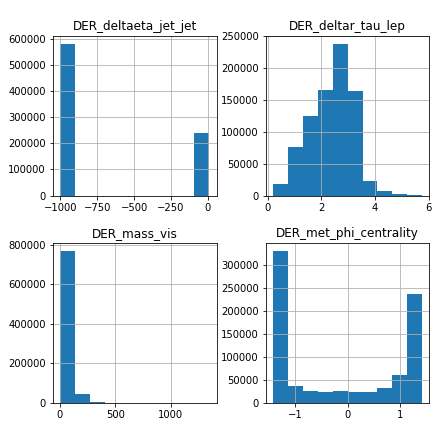
\includegraphics[width=0.5\textwidth]{images/histograms_sample.png}
    \caption{Histogrammes de répartition des valeurs de quelques variables}
    \label{img:hist-sample}
\end{figure}

Afin d’obtenir des \textbf{distributions normales} et de \textbf{stabiliser la
variance}, nous effectuons une \textbf{log-transformation} de manière
indépendante sur les colonnes. Nous commençons par ajouter une constante à
chaque colonne à transformer pour que la valeur minimale de sur cette colonne
soit 1 (comme le log ne prend que des valeurs strictement positives). Nous
appliquons ensuite la fonction log sur les colonnes. Avec ce dataset et en
utilisant cette méthode, nous obtenons toujours des distribution normales.
Finalement nous \textbf{centrons et réduisons} chaque variable de manière
indépendante car cela facilite généralement l’apprentissage des modèles. \\

%The log transformation is one of the most useful transformations in data
%analysis. It is used as a transformation to normality and as a variance
%stabilizing transformation. A log transformation is often used as part of
%exploratory data analysis in order to visualize (and later model) data that
%ranges over several orders of magnitude.

\begin{figure}[H]
	\centering
    \begin{subfigure}[c]{\textwidth}
        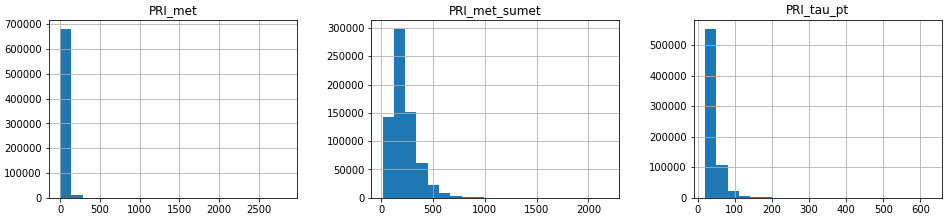
\includegraphics[width=\textwidth]{images/histograms_before_log.png}
    \caption{Avant log-transformation}
    \end{subfigure}

    \begin{subfigure}[c]{\textwidth}
        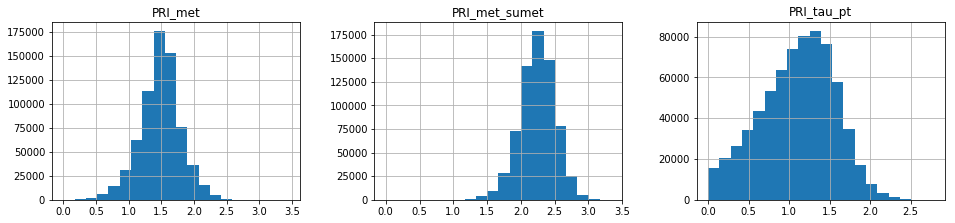
\includegraphics[width=\textwidth]{images/histograms_after_log.png}
    \caption{Après log-transformation}
    \end{subfigure}

    \caption{Histogrammes de répartition des valeurs de quelques variables avant
    et après log-transformation}
    \label{fig:hist-log}
\end{figure}

%Nous
%remarquons cependant que le dataset contient, à vue d'œil, un nombre important
%d'exemples avec des valeurs manquantes (indiquées par -999). Or, travailler avec
%des datasets contenant des données manquantes est compliqué. 

%ous décidons donc
%de supprimer les évènements dont au moins un attribut n'est pas valide et nous
%nous retrouvons avec seulement 223574 exemples : restreindre le dataset aux
%données complètes fait perdre 75\% des données. De plus, la base restreinte
%contient 47\% de signaux, soit 13\% de plus que dans le dataset original. Si ce
%dernier est représentatif de la réalité alors celui restreint ne l'est pas.

\subsection{Valeurs manquantes}

Le dataset contient \textbf{21\% de valeurs manquantes} (indiquées par la valeur
-999).  D’une manière générale, les modèles d’apprentissage statistique ne
gèrent pas automatiquement les valeurs manquantes. Il faut donc traiter ces
données avant de les présenter à nos modèles. Nous considérons trois façons de
pallier à ce problème.

\subsubsection{Omission}

En supprimant les évènements dont au moins un attribut n'est pas valide, nous
retrouvons avec seulement 223574 exemples d’apprentissage : \textbf{restreindre
le dataset aux données complètes fait perdre 75\% des évènements}. Par ailleurs,
la base restreinte contient 47\% de labels positifs, soit 13\% de plus que le
dataset original. Cela met en évidence le fait que les données ne sont pas
manquantes de manière indépendante : l’absence des données est liée à leur
valeur (nous sommes dans un contexte \emph{Missing Not At Random}). Un modèle
entraîné sur le dataset restreint en faisant l’hypothèse "i.i.d." serait donc
biaisé.

\subsubsection{Omission d'attributs}

Une autre méthode consiste à \textbf{supprimer les features dont le pourcentage
de valeurs manquantes dépasse un certain seuil}. On \textbf{retire ensuite les
évènements à valeurs manquantes}. Le dataset final ne contient donc plus aucune
donnée manquante. En fixant le seuil à 40\%, notre jeu de données passe de
818238 à 693636 échantillons, soit 85\% des données initiales, et de 35 à 20
attributs.


\subsubsection{Conservation}

Les \textbf{\emph{Random Forest}} font partie des algorithmes permettant de
\textbf{gérer les données manquantes}. En effet, les arbres de décision peuvent
\textbf{reconnaître une donnée manquante par un simple test de valeur}.

\subsubsection{Affectation (\emph{Imputing})}

Une autre méthode consiste à \textbf{compléter les données manquantes} de la
manière la plus "intelligente" possible. Une fois les données complétées, cela
permet d’\textbf{utiliser tous les modèles de classification à notre
disposition}. 

Nous nous servons de l’algorithme \texttt{IterativeImputing} de
scikit-learn, qui complète de manière itérative les données manquantes en
utilisant des modèles de régression prédisant la valeur d’une variable à partir
de la valeur des autres variables. \\

En pratique et comme nous souhaitons conserver le maximum d'information,
\textbf{nous ne supprimerons ni d'évènements ni d'attributs à valeurs
manquantes}. Nous testerons, d'un côté, des \textbf{algorithmes permettant de
gérer les données manquantes} et, de l'autre, la méthode de \textbf{complétion
des données}. Pour cette dernière, nous appliquons d'abord les
\textbf{log-transformations} puis nous réalisons l’\textbf{imputing} avant de
finir par \textbf{scaler} les données. Ce choix se justifie premièrement par
l’intuition que l’imputing fonctionnera mieux sur des données log-transformées
et, deuxièmement, par le fait qu’estimer la moyenne et la variance en ignorant
les données manquantes serait biaisé.

\subsection{Sélection de features}

Les données sont représentées par \textbf{30 variables explicatives}. Ce nombre
n’étant \textbf{pas très élevé} (par exemple comparé au nombre de pixels dans
une image), il n’y a donc \textbf{pas de grand risque de sur-apprentissage} pour
les modèles. Ainsi, la sélection de caractéristique ne semble pas nécessaire.
Cependant, comme le montre la \figref{img:corr-mat}, certaines variables sont
\textbf{fortement corrélées} (e.g. \texttt{DER\_mass\_MMC} et
\texttt{DER\_mass\_transverse\_met\_lep}), on comparera donc les performances
avec ou sans l’utilisation d’une \textbf{\emph{Analyse en Composantes
Principales} (PCA)} afin de réduire le nombre de données explicatives.

\begin{figure}[H]
    \center
    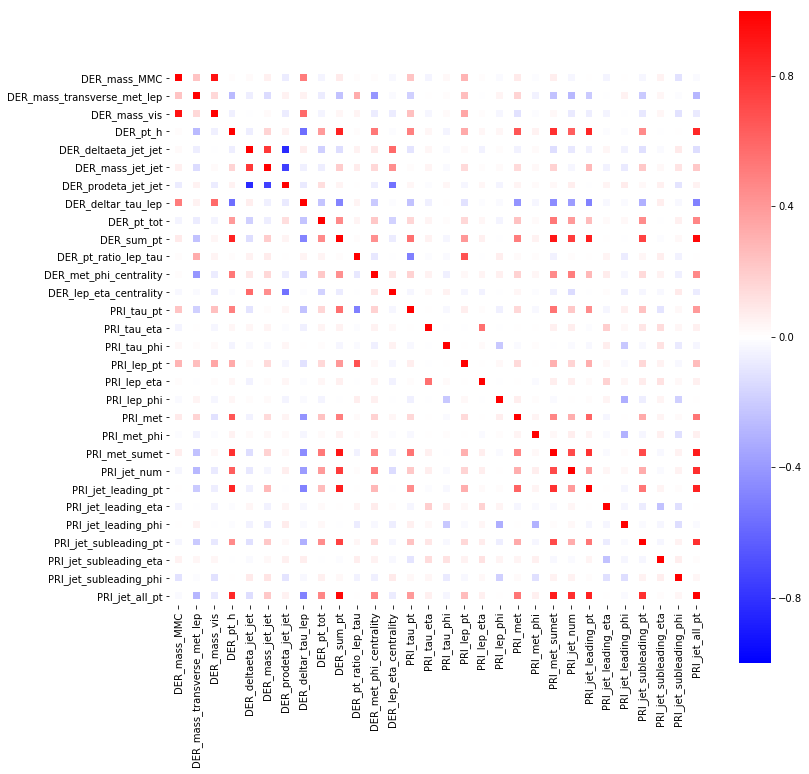
\includegraphics[width=0.7\textwidth]{images/correlation_matrix.png}
    \caption{Matrice de corrélation entre chaque attribut}
    \label{img:corr-mat}
\end{figure}

\section{Classification des évènements}

\subsection{Modèles utilisés}

Nous considérons plusieurs modèles d'apprentissage pour classifier les
évènements :

\begin{itemize}
    \item SVM
    \item méthodes ensemblistes : Bagging de Perceptron, Random Forest, AdaBoost
\end{itemize}

\subsubsection{Support Vector Machines}

Les \emph{Support Vector Machines} (SVMs) nous fournissent une
\textbf{\emph{baseline}}. Généralisation des classifieurs linéaires, ils
nécessitent un \textbf{faible nombre d'hyperpararamètres}, ont des
\textbf{garanties théoriques} et donnent de \textbf{bons résultats} en pratique.

\subsubsection{Méthodes d'ensemble}

Afin de \textbf{réduire de réduire le biais et la variance} de nos modèles et
ainsi améliorer les performances, nous utilisons des \textbf{méthodes
d'ensemble}. Ces algorithmes consistent à \textbf{combiner plusieurs classifieurs
faibles} pour obtenir un modèle \textbf{plus stable, plus robuste et ayant une meilleure
capacité de généralisation}. \\

\textbf{Bootstrap AGGregatING (Bagging). } \quad Le \emph{Bootstrap
Aggregating} est une méthode pour \textbf{réduire la variance par moyennage}.
Plusieurs ensembles d'apprentissage sont simulés par \textbf{\emph{bootstrap} (tirage
avec remise)} puis \textbf{sur chaque sous ensemble, on entraîne un classifieur faible}.
Dans notre contexte de classification binaire, la prédiction du modèle
est définie par le \textbf{vote majoritaire des modèles simples (\emph{bagging})} .

Comme chaque classifieur faible est entraîné sur des données légèrement
différentes, le modèle d'ensemble est capable de \textbf{capturer de petites
variations dans les données} et donc de mieux \textbf{généraliser}. 

Nous choisissons, uniquement pour le Bagging, le \textbf{Perceptron} comme
classifieur faible. Il s'agit d'un \textbf{modèle instable}, ce qui permet
d'obtenir un \textbf{ensemble de classifieurs suffisamment différents}. \\

\textbf{Random Forest. } \quad Avec la technique du Bagging, même si chaque classifieur
est appris sur un jeu de données légèrement différent, tous les modèles se servent des
mêmes attributs pour partitionner les données, les arbres générés
risquent donc d'être \textbf{trop similaires}. Pour pallier à ce problème, les
arbres des \textbf{forêts aléatoires (\emph{random forests})}, également appris
sur des bootstrap de l'ensemble original, \textbf{sélectionnent pour chaque sous ensemble
un échantillon aléatoire de features}, ce qui \textbf{force les modèles à être
différents} et empêche le modèle global de se concentrer sur des attributs particuliers. \\

\textbf{AdaBoost. } \quad Avec la technique de Bagging, les classifieurs faibles
sont appris indépendamment les uns des autres. Or, si ce classifieur est, à lui
seul, trop faible, \textbf{le Bagging ne permettra pas d'obtenir un meilleur
biais}. Le \textbf{\emph{Boosting}} permet de traiter ce problème par
\textbf{apprentissage successif de classifieurs faibles} : en donnant plus de
poids aux exemples mal classés par les modèles précédents, \textbf{chaque nouveau
classifieur se focalise sur les parties de l'espace mal prédites}. Contrairement
au Bagging, la contribution d'un classifieur à la prédiction du modèle
d'ensemble est déterminée par sa performance.

En revanche, si le classifieur faible est trop complexe, le modèle de Boosting
\textbf{risque de sur-apprendre}, auquel cas la technique de Bagging est plus
adaptée.\\

\subsection{Protocole d'expérimentation}


Avant d'entraîner nos modèles, nous pré-traitons l'ensemble de nos données tel que décrit
précédemment (log-transformation, imputing et scaling). \\

Par souci de temps de calcul, les expériences sont menées sur le
dataset restreint à 10000 évènements. 70\% de cette base est dédiée à
l'entraînement et la validation des modèles, 30\% au test.  \\

Pour chaque algorithme, nous procédons par \emph{grid search} pour trouver les
hyperparamètres optimaux. Pour chaque combinaison d'hyperparamètres, le score de
prédiction est estimé par \emph{cross-validation} sur l'ensemble
d'apprentissage. Nous récupérons le classifieur ayant produit le meilleur
résultat et l'évaluons sur les données de test. La seule métrique
utilisée est l'AMS. 

\subsection{Résultats et analyse}

\begin{table}[H]
\centering
\resizebox{0.25\textwidth}{!}{
\begin{tabular}{c|c}
    $C$ & Noyau\\
    \hline
    3.16 & rbf \\
\end{tabular}}
\caption{Paramètres optimaux pour le SVM (accuracy, $n=1000$)}
\end{table}

\begin{table}[H]
\centering
\resizebox{0.8\textwidth}{!}{
\begin{tabular}{c|c|c|c|c}
    & Bagging & RF & RFNan & AdaBoost \\
    \hline
    Profondeur maximale &\cellcolor{gray!40} & 50 & $\inf$ & \cellcolor{gray!40}\\
    Nombre d'estimateurs  & 500 & 500 & 500 & 1000\\
\end{tabular}}
\caption{Paramètres optimaux pour les méthodes d'ensemble (accuracy, $n=1000$)}
\end{table}


\begin{table}[H]
    \resizebox{\textwidth}{!}{
        \begin{tabular}{c|*{3}{c|}c}
            \multirow{2}{*}{} &
            \multicolumn{2}{c|}{Accuracy} &
            \multicolumn{2}{c}{AMS}\\ \cline{2-3} \cline{4-5}
            & Apprentissage & Test & Apprentissage & Test \\
            \hline
            SVM & $75.20 \pm 1.55$ \% & $75.30 \pm 0.42$ \%& & \\
            Bagging & $73.30 \pm 1.24$ \% & $71.80 \pm 0.71$ \% & & \\ 
            RFNan & $81.70 \pm 0.17$ \% & $81.40 \pm 0.82$ \%& & \\
            RF & $80.20 \pm 0.50$ \% & $80.70 \pm 0.62 $\% & & \\
            AdaBoost & $74.30 \pm0.79$ \% & $74.50 \pm 0.58$ \%& &\\
        \end{tabular}}
    \caption{Performances obtenues par chaque méthode}
    \label{tab:ensemble-results}
\end{table}

\todo[inline, color=yellow!40]{Tableaux, graphiques, courbe ROC}


\newpage
\printbibliography
\end{document}

